\documentclass[11pt,a4paper]{article}
\usepackage[margin=1in]{geometry}
\usepackage{amsmath,amssymb,enumitem,fancyhdr,booktabs,listings,tikz,microtype}
\usepackage{needspace}
\usepackage{xcolor}
\usepackage[colorlinks=true,linkcolor=blue]{hyperref}
\pagestyle{fancy}\fancyhf{}
\lhead{\small CSCI-GA.1170-003 Fundamental Algorithms}
\rhead{\small Problem Set 4}\cfoot{PS 4, Page \thepage}
\setlength{\headheight}{14pt}\setlength{\parindent}{0pt}\setlength{\parskip}{0.5em}
\lstset{basicstyle=\ttfamily\small,numbers=left,numberstyle=\tiny,
 numbersep=8pt,xleftmargin=1.5em,columns=fullflexible,keepspaces=true,
 showstringspaces=false,tabsize=4,breaklines=false,frame=single}
\newcommand{\parttitle}[1]{\Needspace{10\baselineskip}\subsection*{#1}}
\newcommand{\proc}[1]{\textsc{#1}}
\begin{document}
\begin{center}
{\Large\bfseries CSCI-GA.1170-003 Fundamental Algorithms\\[0.3em]Problem Set 4}
\end{center}
\noindent\begin{minipage}[t]{0.5\textwidth}
Varun Sahni\\N10338688\\NetID: vs3606
\end{minipage}\begin{minipage}[t]{0.5\textwidth}
\raggedleft October 7, 2026
\end{minipage}

\section*{Problem 4-1 (Heaps: Beyond the Maximum)}
\parttitle{(a) Third largest key}
The largest key is at the root. The larger root child is the second largest. The third largest is the maximum of the other root child and the existing children of the second largest.
\Needspace{22\baselineskip}
\begin{lstlisting}
FIND-3RD-MAX(S):
    heapSize <- |S|
    if heapSize < 3:
        error "The heap must contain at least three keys"
    if S[2] > S[3]:
        secondIndex <- 2
        otherIndex <- 3
    else:
        secondIndex <- 3
        otherIndex <- 2
    thirdLargest <- S[otherIndex]
    leftChildIndex <- Left(secondIndex)
    rightChildIndex <- Right(secondIndex)
    if leftChildIndex <= heapSize:
        thirdLargest <- max(thirdLargest, S[leftChildIndex])
    if rightChildIndex <= heapSize:
        thirdLargest <- max(thirdLargest, S[rightChildIndex])
    return thirdLargest
\end{lstlisting}
Here $\proc{Left}(i)=2i$ and $\proc{Right}(i)=2i+1$ return \emph{indices}. A child exists exactly when its index is at most $\mathtt{heapSize}$. Read $S[\mathtt{leftChildIndex}]$ or $S[\mathtt{rightChildIndex}]$ only after its corresponding existence check succeeds.

\textbf{Correctness.} Every descendant is smaller than its ancestors. Hence the larger root child is second largest. After excluding the root and that child, all remaining nodes belong to the subtree of the other root child or to one of the second largest's child subtrees. Each subtree's maximum is its root. Taking the maximum of these at most three candidate roots therefore returns the third largest. The heap is unchanged.

\textbf{Time and space.} One comparison identifies the second largest, and at most two more compare candidate keys. All other work is constant. Time is $\boxed{\Theta(1)}$ and auxiliary space is $\boxed{O(1)}$, versus $1+4\log n$ for the given naive algorithm.

\Needspace{24\baselineskip}
\textbf{Example.} In $S=(100,90,85,88,70,80,60,75,65)$, the second largest is 90 at index 2. The candidates are 85 at index 3, 88 at index 4, and 70 at index 5. The answer changes from $85$ to $88$, then stays $88$.
\begin{center}
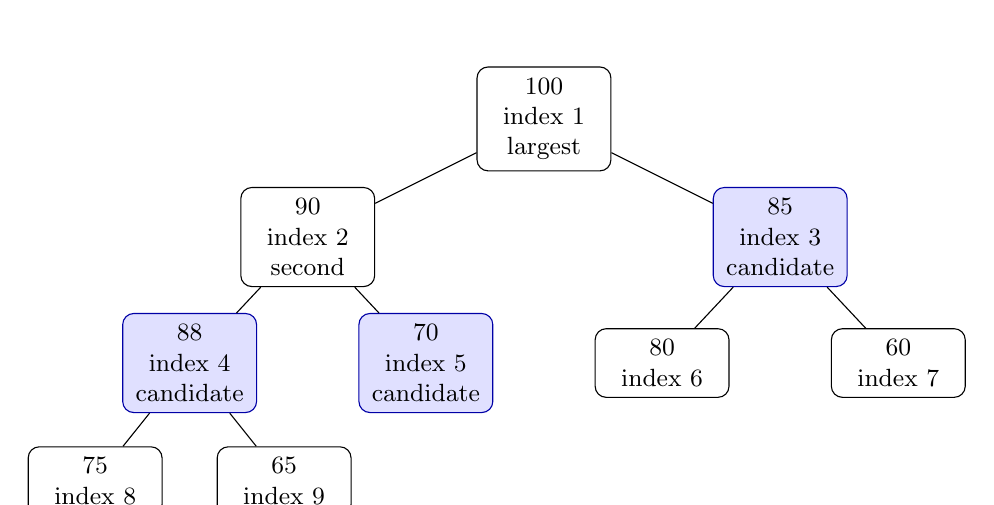
\begin{tikzpicture}[
 every node/.style={draw,rounded corners,align=center,font=\small,minimum width=17mm,inner sep=4pt},
 candidate/.style={fill=blue!12,draw=blue!65!black}]
\node (root) at (0,0) {$100$\\index 1\\largest};
\node (second) at (-3,-1.5) {$90$\\index 2\\second};
\node[candidate] (other) at (3,-1.5) {$85$\\index 3\\candidate};
\node[candidate] (left) at (-4.5,-3.1) {$88$\\index 4\\candidate};
\node[candidate] (right) at (-1.5,-3.1) {$70$\\index 5\\candidate};
\node (six) at (1.5,-3.1) {$80$\\index 6};
\node (seven) at (4.5,-3.1) {$60$\\index 7};
\node (eight) at (-5.7,-4.6) {$75$\\index 8};
\node (nine) at (-3.3,-4.6) {$65$\\index 9};
\draw (root)--(second) (root)--(other)
 (second)--(left) (second)--(right) (other)--(six) (other)--(seven)
 (left)--(eight) (left)--(nine);
\end{tikzpicture}
\end{center}
The blue nodes are the only candidates. Each other remaining node is below a candidate and is smaller than it.

\parttitle{(b) Replace-Max}
The naive algorithm removes the maximum and inserts the replacement. The intelligent algorithm replaces the root directly, then repairs downward.
\Needspace{14\baselineskip}
\begin{lstlisting}
REPLACE-MAX-NAIVE(S, replacementKey):
    if |S| == 0: error "The heap is empty"
    originalMaximum <- Extract-Max(S)
    Insert(S, replacementKey)
    return originalMaximum

REPLACE-MAX-INTELLIGENT(S, replacementKey):
    if |S| == 0: error "The heap is empty"
    originalMaximum <- S[1]
    S[1] <- replacementKey
    Max-Heapify(S, 1)
    return originalMaximum
\end{lstlisting}
\textbf{Correctness.} Extraction and insertion keep a valid heap and replace exactly the original maximum. In the intelligent version, the child subtrees stay valid when the root changes. Only the root's comparisons with its children can fail, so max-heapify restores heap order. Both algorithms return the saved original maximum and keep every other key.

\textbf{Time.} Under the given operation costs, the naive version costs $2\log n+O(1)$ and the intelligent version costs $\log n+O(1)$: two heap repairs versus one. Both have $O(\log(n+1))$ worst-case time. The intelligent version takes $\Theta(1)$ if the new root already dominates its children. For $n=1$, both take constant time.

\textbf{Space.} Both use $O(1)$ auxiliary space with iterative heap operations. A recursive implementation of heapify uses $O(\log(n+1))$ stack space.

\parttitle{(c) Report-Greater}
\textbf{Naive algorithm.} Repeatedly extract the maximum while it exceeds the threshold. Save the extracted keys, then reinsert them to restore the queue.
\Needspace{15\baselineskip}
\begin{lstlisting}
REPORT-GREATER-NAIVE(S, threshold):
    reportedKeys <- empty list
    remainingCount <- |S|
    while remainingCount > 0:
        if Maximum(S) <= threshold:
            break
        append Extract-Max(S) to reportedKeys
        remainingCount <- remainingCount - 1
    for each reportedKey in reportedKeys:
        Insert(S, reportedKey)
    return reportedKeys
\end{lstlisting}
\textbf{Correctness.} After each extraction, the list contains exactly the removed largest keys, all greater than the threshold. On stopping, the heap is empty or its maximum is at most the threshold, so every required key has been reported. Reinsertion restores the original keys. As a priority queue, $S$ is unchanged; its internal array order may differ.

\textbf{Time and space.} For $m$ reported keys there are $m$ extractions, $m$ insertions and at most $m+1$ maximum tests. The given primitive costs give $\boxed{\Theta(1+m\log(n+1))}$ time. This also accounts for shrinking heap sizes: if $m\le n/2$, the extraction sizes are at least $n/2$; if $m>n/2$, at least $\lfloor n/2\rfloor$ extractions have that size and $m=\Theta(n)$. The saved output uses $O(m)$ space; iterative primitives need $O(1)$ additional space.

\textbf{Intelligent algorithm.} Start at the root. Report a key greater than the threshold and visit its children. Otherwise skip the entire subtree, since its descendants are no larger.
\Needspace{18\baselineskip}
\begin{lstlisting}
REPORT-GREATER-INTELLIGENT(S, threshold):
    reportedKeys <- empty list
    VISIT(S, 1, threshold, reportedKeys)
    return reportedKeys

VISIT(S, nodeIndex, threshold, reportedKeys):
    if nodeIndex > |S|:
        return
    if S[nodeIndex] <= threshold:
        return
    append S[nodeIndex] to reportedKeys
    VISIT(S, Left(nodeIndex), threshold, reportedKeys)
    VISIT(S, Right(nodeIndex), threshold, reportedKeys)
\end{lstlisting}
\textbf{Correctness.} Induct on subtree height. A missing node contributes nothing. A root at most the threshold has no qualifying descendants, so pruning is correct. Otherwise the root qualifies, and the recursive calls report exactly the qualifying keys in its two disjoint child subtrees by induction. Each key is reported once. The algorithm never writes to $S$, so even its array order is unchanged.

\textbf{Time and space.} Each reported node creates two child calls; the initial root call adds one. Thus there are exactly $2m+1$ calls, each with constant work, giving $\boxed{\Theta(m+1)}$ time independent of $n$. The output uses $O(m)$ space. The recursion stack uses $O(1+\min\{m,\log(n+1)\})$ auxiliary space.

\parttitle{(d) Decrease-Key}
The naive algorithm replaces the selected key by $+\infty$, extracts it, then inserts the decreased value. Here $+\infty$ is a temporary key larger than every valid key. The intelligent algorithm writes the decreased value and repairs downward.
\Needspace{12\baselineskip}
\begin{lstlisting}
DECREASE-KEY-NAIVE(S, keyIndex, decreasedKey):
    Increase-Key(S, keyIndex, +infinity)
    Extract-Max(S)                // discard the sentinel
    Insert(S, decreasedKey)

DECREASE-KEY-INTELLIGENT(S, keyIndex, decreasedKey):
    S[keyIndex] <- decreasedKey
    Max-Heapify(S, keyIndex)
\end{lstlisting}
Both procedures assume a valid index and $\mathtt{decreasedKey}<S[\mathtt{keyIndex}]$ before the change.

\textbf{Correctness.} The naive version removes exactly the selected original key: increase-key moves its sentinel upward, and extract-max removes that sentinel. Insertion then puts the decreased key into a valid heap. The intelligent version preserves the parent inequality, since decreasing a key cannot make it exceed its parent. Its child subtrees remain valid, so max-heapify repairs the only possible violations.

\textbf{Time and space.} The naive version costs $3\log n+O(1)$ in the stated model; the intelligent version costs at most $\log n+O(1)$. Both have $O(\log(n+1))$ worst-case time and $O(1)$ auxiliary space with iterative primitives. More precisely, intelligent repair costs $O(h+1)$ for a node of height $h$, so a leaf takes $\Theta(1)$. Recursive heapify uses $O(h+1)$ stack space.

\textbf{Why not use heapify for increase-key?} Increasing a key can make it larger than its parent. Heapify compares only with children, so it cannot repair that upward violation. Increase-key must move the key upward instead.

\newpage
\section*{Problem 4-2 (Quicksort vs Heapsort on Nice Arrays)}
For distinct keys, $c$-niceness means $A[i]<A[j]$ whenever $j-i\ge c$. Ranks count from 1 for the smallest element. We take $c$ to be a fixed positive integer.

\parttitle{(a) Rank bounds}
The rank of $A[i]$ is its position in the fully sorted array: rank 1 is the smallest key, rank 2 the second smallest, and so on. Thus
\[
\operatorname{rank}(A[i])=1+\#\{\text{keys smaller than }A[i]\}.
\]
We use $c$-niceness to count keys that must be smaller or larger.

\textbf{Lower bound.} Positions $1,\ldots,i-c$ are at least $c$ positions to the left of $i$, so their keys must be smaller than $A[i]$. There are $\max\{0,i-c\}$ such keys. Adding one gives rank at least $\max\{1,i-c+1\}$.

\textbf{Upper bound.} Positions $i+c,\ldots,n$ must contain larger keys. There are $\max\{0,n-i-c+1\}$ of them, so the rank is at most $n-\max\{0,n-i-c+1\}=\min\{n,i+c-1\}$. Therefore
\[
\boxed{\max\{1,i-c+1\}\le\operatorname{rank}(A[i])
\le\min\{n,i+c-1\}.}
\]
To prove that these are the best bounds, start with the sorted array $(1,2,\ldots,n)$, where each value equals its rank. To reach the lower bound, reverse the block from position $\ell=\max\{1,i-c+1\}$ to position $i$. This puts value $\ell$ at position $i$, giving rank $\ell$. To reach the upper bound, start again with the sorted array and reverse the block from position $i$ to position $u=\min\{n,i+c-1\}$. This puts value $u$ at position $i$, giving rank $u$.

Each reversed block has at most $c$ entries. The only pairs put out of order are inside that block, so their positions differ by less than $c$. Both arrays therefore remain $c$-nice, and neither bound can be improved.

Now assume the pivot is the first entry $A[p]$ of each current subarray $A[p..r]$. After partitioning, it is at index $q$; quicksort continues on $A[p..q-1]$ and $A[q+1..r]$. 

\parttitle{(b) Both subarrays remain $c$-nice}
Consider the first partition of $A[1..n]$, with pivot $x=A[1]$ and final pivot index $q$. We must show that \emph{within each resulting part}, any two entries at least $c$ positions apart are in increasing order.

\textbf{Where swaps occur.} By (a), the first entry has rank at most $c$, so $q\le c$. Also, original positions $c+1,\ldots,n$ contain keys larger than $x$. Thus the scan encounters smaller keys only in positions $2..c$, and every swap stays within the first $c$ positions. Entries after position $c$ are unchanged.

\textbf{Left part $A[1..q-1]$.} It has $q-1\le c-1$ entries. No pair of its indices is $c$ positions apart, so it satisfies the definition of $c$-niceness automatically.

\textbf{Right part $A[q+1..n]$.} In the scan, a key larger than $x$ can only stay in place or move right when exchanged with a smaller key. The final pivot swap touches positions 1 and $q$, outside the right part.

Take any final right-part positions $u<v$ with $v-u\ge c$. Since $u\ge q+1\ge2$, we have $v>c$, so the key at $v$ is unchanged. The key now at $u$ came from an original position $a\le u$. Therefore $v-a\ge v-u\ge c$. Original $c$-niceness gives
\[
A_{\mathrm{after}}[u]=A_{\mathrm{before}}[a]
<A_{\mathrm{before}}[v]=A_{\mathrm{after}}[v].
\]
This proves the required order for every such pair in the right part. Hence both resulting subarrays are $c$-nice. Reindexing a subarray leaves index distances unchanged, so the same argument applies at later recursive calls.

A partition scans $n-1$ entries, so it takes $\Theta(n)$ time and $O(1)$ auxiliary space. The full quicksort analysis follows in (c).

\parttitle{(c) Best-case running time}
By (a), a first-position pivot has rank at most $c$. Therefore its left part has size $s\le c-1$, and its right part has size $n-s-1\ge n-c$. By (b), both children are still $c$-nice. For any run, its time recurrence at a node is
\[
T(A)=T(A_L)+T(A_R)+\Theta(n),
\qquad |A_L|=s\le c-1,\quad |A_R|=n-s-1.
\]
Let $B_c(n)$ denote the minimum runtime over all $c$-nice arrays of length $n$. Each child takes at least the best-case time for its size. Therefore
\[
B_c(n)\ge
\min_{0\le s\le\min\{c-1,n-1\}}
\{B_c(s)+B_c(n-s-1)\}+\alpha(n-1),
\]
for a fixed $\alpha>0$ accounting for the scan comparisons, with constant base costs. This is a lower bound because the two child minima need not occur together.

Follow the right child after each partition. After $j$ partitions its size is at least $n-jc$. Let $d=\lfloor n/(2c)\rfloor$. Each of the first $d$ partitions handles at least $n/2$ entries, so
\[
B_c(n)\ge\alpha\sum_{j=0}^{d-1}(n-jc-1)
=\alpha\left(d(n-1)-\frac{cd(d-1)}2\right)
=\Omega(n^2/c).
\]
For fixed $c$, this is $\Omega(n^2)$.

Quicksort is $O(n^2)$ on every array: at depth $d$ its active subarrays are disjoint, their total size is at most $n$, and depth is at most $n$. A sorted array is also $c$-nice and has $T(n)=T(n-1)+\Theta(n)=\Theta(n^2)$, giving the same quadratic bound. Therefore
\[
\boxed{B_c(n)=\Theta(n^2)\quad\text{for fixed }c.}
\]
The constants may depend on $c$. Standard recursive quicksort uses $\Theta(n)$ stack space for fixed $c$: the right-child chain loses at most $c$ entries per call, so it has $\Omega(n/c)$ depth; no chain exceeds $n$. Each partition uses $O(1)$ extra space. 

\Needspace{25\baselineskip}
\parttitle{(d) Sort-Nice}
Use a min-heap containing at most $b$ candidates. Build it from the first $b$ entries. Repeatedly output its minimum and insert the next unread entry, if one remains.

\textbf{Min-heap procedures.} Use the CLRS heap procedures with comparisons reversed. The array $H$ has capacity $H.\mathtt{length}$ and active size $H.\mathtt{heapSize}$. Its parent and child indices are
\[
\proc{Parent}(i)=\lfloor i/2\rfloor,\qquad
\proc{Left}(i)=2i,\qquad \proc{Right}(i)=2i+1.
\]
Min-heap order means each parent key is at most its children's keys. Therefore $H[1]$ is the minimum.

\Needspace{25\baselineskip}
\begin{lstlisting}
MIN-HEAPIFY(H, nodeIndex):
    leftIndex <- Left(nodeIndex)
    rightIndex <- Right(nodeIndex)
    smallestIndex <- nodeIndex
    if leftIndex <= H.heapSize:
        if H[leftIndex] < H[smallestIndex]:
            smallestIndex <- leftIndex
    if rightIndex <= H.heapSize:
        if H[rightIndex] < H[smallestIndex]:
            smallestIndex <- rightIndex
    if smallestIndex != nodeIndex:
        exchange H[nodeIndex] and H[smallestIndex]
        MIN-HEAPIFY(H, smallestIndex)

BUILD-MIN-HEAP(H):
    H.heapSize <- H.length
    for nodeIndex <- floor(H.length / 2) downto 1:
        MIN-HEAPIFY(H, nodeIndex)
\end{lstlisting}
\textbf{Heapify correctness.} Assume both child subtrees are min-heaps. If the current key is smallest, the subtree is already valid. Otherwise swap it with the smaller child. The new root is no larger than either child; only the chosen child's subtree may now need repair. Induction on height proves the recursive call restores that subtree. Each call moves down one level, so time and stack space are $O(\log(m+1))$ for an $m$-entry heap.

\textbf{Build correctness and time.} Before each iteration, every higher-indexed node roots a min-heap. Initially these nodes are leaves. Since children have larger indices than their parent, heapify's assumption holds and the iteration establishes the invariant for the next node. At termination, the root is a min-heap. Nodes of height $h$ number at most $\lceil m/2^{h+1}\rceil$; summing their $O(h+1)$ repair costs gives $O(m)$, since $\sum_{h\ge0}(h+1)/2^h$ is constant (the rounding terms add $O(\log^2(m+1))=O(m)$). Thus build time is $\Theta(m)$. It modifies the array in place and uses $O(\log(m+1))$ stack space for recursive heapify.

\Needspace{13\baselineskip}
\begin{lstlisting}
HEAP-EXTRACT-MIN(H):
    if H.heapSize == 0:
        error "The heap is empty"
    minimumKey <- H[1]
    H[1] <- H[H.heapSize]
    H.heapSize <- H.heapSize - 1
    if H.heapSize > 0:
        MIN-HEAPIFY(H, 1)
    return minimumKey
\end{lstlisting}
The root is the minimum. Replacing it by the last key and shrinking the active size leaves both child subtrees valid, so heapify restores min-heap order. This takes $O(\log(m+1))$ time and recursive stack space.

\Needspace{20\baselineskip}
\begin{lstlisting}
HEAP-DECREASE-KEY(H, keyIndex, newKey):
    if newKey > H[keyIndex]:
        error "The new key must not increase"
    H[keyIndex] <- newKey
    while keyIndex > 1:
        parentIndex <- Parent(keyIndex)
        if H[parentIndex] <= H[keyIndex]:
            break
        exchange H[keyIndex] and H[parentIndex]
        keyIndex <- parentIndex

MIN-HEAP-INSERT(H, newKey):
    H.heapSize <- H.heapSize + 1
    H[H.heapSize] <- +infinity
    HEAP-DECREASE-KEY(H, H.heapSize, newKey)
\end{lstlisting}
Decrease-key moves the changed key upward while it is smaller than its parent. Only that parent edge can violate heap order, and each swap moves the possible violation one level upward. It stops at the root or a valid parent edge. Insert adds a leaf with temporary key $+\infty$, then decreases it to the new key. Both take $O(\log(m+1))$ time and $O(1)$ extra space. In Sort-Nice, insertion always follows extraction, so the capacity $b$ is sufficient.

\textbf{Sort-Nice.} Here $\mathtt{windowSize}=b$ and $\mathtt{arraySize}=n$. Write $B$ for the returned output array. The input $A$ stays unchanged, so later trials can reuse it.
\Needspace{16\baselineskip}
\begin{lstlisting}
SORT-NICE(A, windowSize):
    arraySize <- |A|              // 1 <= windowSize <= arraySize
    candidateHeap <- copy of A[1..windowSize]
    BUILD-MIN-HEAP(candidateHeap)
    sortedOutput <- new array of length arraySize
    nextInputIndex <- windowSize + 1
    for outputIndex <- 1 to arraySize:
        minimumKey <- HEAP-EXTRACT-MIN(candidateHeap)
        sortedOutput[outputIndex] <- minimumKey
        if nextInputIndex <= arraySize:
            MIN-HEAP-INSERT(candidateHeap, A[nextInputIndex])
            nextInputIndex <- nextInputIndex + 1
    return sortedOutput
\end{lstlisting}
\textbf{Permutation guarantee for every input.} Each original entry is inserted exactly once: the first $b$ at construction and all remaining entries through $\mathtt{nextInputIndex}$. At output position $t=\mathtt{outputIndex}$, the heap contains exactly the inserted entries not yet output. It is nonempty until all $n$ iterations finish. Each extraction removes one entry and appends that entry exactly once to $B$. After $n$ outputs nothing remains; $B$ is a permutation, regardless of niceness or the choice of $b$.

\textbf{Sortedness when $c\le b$.} Induct on output position $t$. Assume the first $t-1$ outputs are the globally smallest $t-1$ entries in order. Immediately before extraction $t$, all entries through original position $\min\{n,t+b-1\}$ have been inserted. By (a), an entry of global rank $t$ has original position
\[
i\le t+c-1\le t+b-1.
\]
It has therefore been inserted, and it has not yet been output. It is in the heap and is the smallest remaining original entry. Extract-min returns it. The initial case $t=1$ follows from the same inequality; induction proves the output sorted.

\textbf{Running time.} Building costs $O(b)$. There are $n$ extractions and $n-b$ insertions on heaps of size at most $b$, plus $O(n)$ output/bookkeeping:
\[
T(n,b)=O\bigl(b+n+(2n-b)\log(b+1)\bigr)
=\boxed{O\bigl(n\log(b+1)\bigr)}.
\]
For $b\ge2$ this is the requested $O(n\log b)$; for $b=1$ it is $\Theta(n)$.  Heap space is $O(b)$, with $O(n)$ output space.

\parttitle{(e) Doubling guesses}
Use $b_i=\min\{n,2^i\}$ to respect (d)'s allowed range, with $i=0,1,\ldots$. Every trial uses the original $A$. Checking whether the trial output is sorted costs $\Theta(n)$ in the worst case. The last trial certainly succeeds at $b=n$, because then all entries are in the heap before any extraction.

If $A$ is $c^*$-nice, put $\widehat c=\min\{c^*,n\}$ and $L=\lceil\log_2\widehat c\rceil$. A trial succeeds no later than $i=L$, since its capacity is at least $\widehat c$. Each trial costs $O(n(1+i))$, including the sortedness scan, so
\[
\begin{aligned}
T(n,c^*)&\le O\!\left(n\sum_{i=0}^{L}(1+i)\right)\\
&=O\!\left(n\left((L+1)+\frac{L(L+1)}2\right)\right)\\
&=\boxed{O\bigl(n(1+\log^2 c^*)\bigr)}.
\end{aligned}
\]
For $c^*\ge2$ this is $O(n\log^2 c^*)$; for $c^*=1$ the first trial returns the already-sorted input in $\Theta(n)$. Earlier success only improves this bound. Space is $O(n)$ when each unsuccessful output is discarded before the next trial.

Reversing an array of size $n=2^L$ gives a family with minimum niceness parameter $c^*=n$. Each trial with $b<n$ outputs $n-b+1$ first and later outputs the unseen value 1, so fails. For powers $b\le n/2$, the remaining unseen descending values are successive new minima and are inserted into a heap of size $b$, requiring $\Theta(\log b)$ upward work per insertion. There are at least $n/2$ such insertions per trial. Hence the trials cost $\Omega(n\sum_{i=1}^{L-1}i)=\Omega(nL^2)$ in total. Thus this schedule can require $\Theta(n\log^2 c^*)$ time.

\newpage
\parttitle{(f) Faster guesses}
After testing $b=1$, use guesses $2,4,16,256,\ldots$, squaring the previous guess and capping at $n$.
\Needspace{14\baselineskip}
\begin{lstlisting}
NICE-BUT-WEIRD-SORT-FAST(A):
    arraySize <- |A|              // requires arraySize >= 1
    windowSize <- 1
    while true:
        sortedOutput <- SORT-NICE(A, windowSize)
        if IS-SORTED(sortedOutput):
            return sortedOutput
        if windowSize == 1:
            windowSize <- min(arraySize, 2)
        else:
            windowSize <- min(arraySize, windowSize * windowSize)
\end{lstlisting}
\textbf{Correctness and termination.} Every trial output is a permutation. The algorithm returns only a sorted one. A failed trial with $b<n$ increases $b$ strictly; a trial at $b=n$ always succeeds. Thus termination and correctness follow without knowing $c^*$.

For $c^*>1$, if the successful trial is not the first $b=2$ trial, its previous guess was below $\widehat c$: otherwise (d) would already have guaranteed success. The last capacity is therefore at most $\widehat c^2$ (or the smaller cap $n$), so its logarithm is less than $2\log_2\widehat c$. Before capping, the positive logarithms are $1,2,4,8,\ldots$. Their sum is at most twice the largest one. The number of sortedness checks is also at most a constant plus this sum. Consequently
\[
\boxed{T(n,c^*)=O\bigl(n(1+\log c^*)\bigr)}.
\]
For $c^*\ge2$, this is the requested $O(n\log c^*)$; for $c^*=1$, it is $\Theta(n)$. Space is $O(n)$, discarding each failed trial before the next.

\newpage
\section*{Problem 4-3 (Assigning Letter Grades)}
A score $s$ belongs to band $j$ exactly when $c_{j-1}<s\le c_j$. The finite cutoffs $c_1<\cdots<c_{k-1}$ are already ordered. Sorting inside a band is unnecessary.

\parttitle{(a) Randomized quicksort and Partition-Value}
Randomized quicksort returns a sorted permutation by the partition postcondition and induction on subarray length. In sorted order, a higher band cannot precede a lower band: if $s$ belongs to band $a$ and $t$ to band $b>a$, then $s\le c_a\le c_{b-1}<t$. Therefore sorting solves the grouping problem.

Lecture randomized quicksort has expected time $\boxed{O(n\log n)}$, so Hari's algorithm has that bound. It uses $O(n)$ worst-case recursion-stack space in the standard implementation.

\textbf{Partition-Value.} Since $c$ need not be an entry, scan \emph{all} entries, do not reserve a pivot slot, and do not perform a final pivot exchange.
\Needspace{10\baselineskip}
\begin{lstlisting}
PARTITION-VALUE(A, startIndex, endIndex, cutoffValue):
    lowerEnd <- startIndex - 1
    for scanIndex <- startIndex to endIndex:
        if A[scanIndex] <= cutoffValue:
            lowerEnd <- lowerEnd + 1
            exchange A[lowerEnd] and A[scanIndex]
    return lowerEnd
\end{lstlisting}
\textbf{Invariant.} Write $p=\mathtt{startIndex}$, $r=\mathtt{endIndex}$, $q=\mathtt{lowerEnd}$, $t=\mathtt{scanIndex}$ and $c=\mathtt{cutoffValue}$. Before iteration $t$, $A[p..q]\le c$, $A[q+1..t-1]>c$, and $A[t..r]$ is unprocessed. The subarray remains a permutation of its original entries. Initially both processed regions are empty. If the next entry is at most $c$, incrementing $q$ and exchanging moves it into the low region and the displaced high-region entry (if any) to the end of the high region. Otherwise it simply extends the high region. Thus every branch maintains the invariant. At termination $t=r+1$, it gives
\[
\boxed{A[p..q]\le c<A[q+1..r].}
\]
Exactly $r-p+1$ entries are scanned; time is $\Theta(r-p+1)$ for a nonempty interval and auxiliary space $O(1)$. If none qualify, $q=p-1$; if all qualify, $q=r$. An empty interval returns $p-1$ in constant time. Equality belongs on the left, as the band definition requires.

\parttitle{(b) Mira's sequential cutoffs}
\Needspace{10\baselineskip}
\begin{lstlisting}
SEQUENTIAL-BAND-SORT(A, cutoffs[1..bandCount-1]):
    remainingStart <- 1
    for cutoffIndex <- 1 to bandCount-1:
        if remainingStart > |A|:
            return
        bandEnd <- PARTITION-VALUE(
            A, remainingStart, |A|, cutoffs[cutoffIndex])
        remainingStart <- bandEnd + 1
\end{lstlisting}
\textbf{Correctness.} Before cutoff $c_j$, the completed prefix consists of bands $1,\ldots,j-1$ in order, and every remaining score exceeds $c_{j-1}$. The first step has empty prefix and lower bound $-\infty$. Partitioning the suffix at $c_j$ places exactly the scores in $(c_{j-1},c_j]$, namely band $j$, immediately after that prefix. The new suffix exceeds $c_j$. At the end only band $k$ remains, so all bands are grouped. Swaps preserve all scores. Empty bands create an empty block without invalidating the invariant.

Each of $k-1$ partitions scans at most $n$ entries, with constant loop overhead, so worst-case time is $O(nk)$ for $k\ge2$; $k=1$ needs no rearrangement and takes $O(1)$ for this procedure. Auxiliary space is $O(1)$.

\textbf{Tight example.} Let $c_j=j$ for $j=1,\ldots,k-1$ and $A[t]=k+t$ for $t=1,\ldots,n$. All scores lie in band $k$. Every partition returns $\mathtt{lowerEnd}=0$ and leaves $\mathtt{remainingStart}=1$, hence scans all $n$ scores. The total is
\[
(k-1)\Theta(n)=\boxed{\Theta(nk)}\quad(k\ge2).
\]

\parttitle{(c) Band-Sort}
Cutoffs are stored in the shared read-only array $\mathtt{cutoffs}[1..k-1]$, with $\mathtt{cutoffs}[j]=c_j$. The parameters $\mathtt{firstCutoff}=i$ and $\mathtt{lastCutoff}=j$ specify the remaining cutoff indices; $\mathtt{startIndex}=p$ and $\mathtt{endIndex}=r$ specify the score interval. A one-score interval may still need classification, so return only for an empty score interval or no remaining cutoffs.
\Needspace{10\baselineskip}
\begin{lstlisting}
BAND-SORT(A, startIndex, endIndex, firstCutoff, lastCutoff):
    if startIndex > endIndex or firstCutoff > lastCutoff:
        return
    middleCutoff <- floor((firstCutoff + lastCutoff) / 2)
    lowerEnd <- PARTITION-VALUE(
        A, startIndex, endIndex, cutoffs[middleCutoff])
    BAND-SORT(A, startIndex, lowerEnd,
              firstCutoff, middleCutoff-1)
    BAND-SORT(A, lowerEnd+1, endIndex,
              middleCutoff+1, lastCutoff)
\end{lstlisting}
Initial call:
\[
\boxed{\proc{Band-Sort}(A,1,n,1,k-1).}
\]
Here $q=\mathtt{lowerEnd}$ and $m=\mathtt{middleCutoff}$. The left child includes $q$: unlike quicksort, no actual pivot element is removed from the array.

\textbf{Inductive claim.} If every score in $A[p..r]$ lies in $(c_{i-1},c_{j+1}]$, the procedure preserves its multiset and groups it into bands $i,i+1,\ldots,j+1$ in ascending band order. This range invariant is true for the initial call since $c_0=-\infty$ and $c_k=+\infty$. Induct on the number $t=j-i+1$ of remaining cutoffs.

\textbf{Base cases.} An empty score interval is already grouped. If there are no cutoffs, $i=j+1$; the range invariant puts all scores in the single band $i$, so returning is correct.

\textbf{Induction step.} With $t\ge1$ and a nonempty interval, value partition at $c_m$ preserves all scores and yields a left part in $(c_{i-1},c_m]$ and a right part in $(c_m,c_{j+1}]$. The left recursive call uses fewer cutoffs $c_i,\ldots,c_{m-1}$ and satisfies its range precondition; the right call uses fewer cutoffs $c_{m+1},\ldots,c_j$ and satisfies its own. By induction they group bands $i,\ldots,m$ and $m+1,\ldots,j+1$, respectively. Every band on the left precedes every band on the right, and their concatenation is the original interval rearranged in the required order. This proves the claim. The number of remaining cutoffs strictly decreases on each nonbase recursive call, so the procedure terminates even when one score part is empty.

\parttitle{(d) Recursion depth, disjointness and runtime}
A node with $t$ cutoffs gives each child at most $\lfloor t/2\rfloor$ cutoffs: the middle cutoff is removed and the two remaining cutoff counts differ by at most one. Starting with $t=k-1$, a node at depth $d$ has at most
\[
\left\lfloor\frac{k-1}{2^d}\right\rfloor
\]
cutoffs. For $D=\lceil\log_2 k\rceil$, $2^D\ge k>k-1$, so no partition is performed at depth $D$. There are at most $D$ partition levels, and the recursion's edge depth, including base calls, is at most $D$. For $k=1$, this is zero.

\textbf{Disjointness.} The root is the only interval at depth zero. Each interval $[p,r]$ divides into disjoint children $[p,q]$ and $[q+1,r]$ whose union is its parent (empty intervals are allowed). Children of disjoint parents cannot intersect. Induction on depth therefore proves disjointness at every level. Thus their total nonempty length is at most $n$.

At a partition level, scanning costs at most $O(n)$ in total. The constant overhead is also $O(n)$: there are at most $n$ nonempty intervals at that level. Empty child calls add at most twice the number of internal nodes overall, so they do not change the bound. Consequently
\[
\boxed{T(n,k)=O(n\lceil\log_2 k\rceil+1)
=O(n\log k)\quad(k\ge2).}
\]
For $k=1$ the procedure returns immediately in $O(1)$. It uses $O(\log k)$ recursion-stack space and $O(1)$ extra space in each value partition; no separate output array is needed.

For $k=2$, there is one scan and the runtime is $\Theta(n)$, matching Mira and improving on Hari's expected $O(n\log n)$. For $k=n\ge2$, the guarantee is $O(n\log n)$ in the worst case, matching Hari's expected bound while improving on Mira's $O(n^2)$ worst-case bound.

\parttitle{(e) Smallest remaining cutoff}
Choosing the smallest remaining cutoff $c_i$ leaves no cutoffs for the left recursive call, so it returns immediately. Only the right call continues, with one fewer cutoff. There are at most $k-1$ partitions, each taking $O(n)$ time, which gives an upper bound of $O(nk)$.

To show this bound is tight, let every score exceed $c_{k-1}$. Each partition then leaves the left part empty and all $n$ scores in the right part. All $k-1$ partitions therefore scan the entire array. With $t$ remaining cutoffs, the running time on this input satisfies
\[
W(n,t)=W(n,t-1)+\Theta(n),\qquad W(n,0)=\Theta(1).
\]
Thus the worst-case time is
\[
\boxed{W(n,k-1)=\Theta(n(k-1)+1)=\Theta(nk)\quad(k\ge2).}
\]
For $k=1$, there are no cutoffs and the running time is $\Theta(1)$. The recursion stack uses $O(k)$ space and can have $\Theta(k)$ depth.

This resembles \textbf{Mira's sequential algorithm from (b)}: partition around $c_1$, then partition the remaining suffix around $c_2$, and continue in increasing cutoff order.

This is the same unbalanced-partition behavior as quicksort with an extreme pivot, whose recurrence is $T(n)=T(n-1)+\Theta(n)$. Here one cutoff is removed per level while all scores may stay in the right part; in quicksort one pivot is removed per level. For $k=n$, both have quadratic worst-case running time.

\end{document}
